\chapter{Technische Umsetzung (brv)}
\label{chap:technUmsetzung}

	\section{Speicherung der Profildaten}
	\label{sec:speicherungProfildaten}
	
	Profildaten, die der Nutzer in der App eingibt, werden persistent gespeichert. Die Daten werden mit dem Flutter Plugin SQLFlite (\hyperlink{https://pub.dev/packages/sqflite}{https://pub.dev/packages/sqflite}) gespeichert. Das Plugin speichert Daten in einer SQLite Datenbank.
	\\
	Profildaten werden bei jeder Änderung automatisch gespeichert. Hierzu gehört nicht nur das Laden neuer Daten, sondern auch das Verändern von Eingabevariablen und dem Kommentarfeld.
	\\
	Die Datenverwaltung basiert im wesentlichen auf zwei Komponenten:
	
	\begin{itemize}
		\item \textbf{Profilklasse (\textit{profile.dart}):} Die Profilklasse repräsentiert Profile, die in der App gespeichert werden können. Jedes Profil besteht dabei aus einer ID, einem Namen, dem letzten Änderungsdatum, der ID, mit der die Messung vom Server geladen wurde (falls die Messung nicht per QR-Code gescannt wurde), einem Satz von Messwerten, einem Satz von Simulationswerten und dem optionalen Kommentar.
		
		Die Klasse verfügt außerdem über die Methode \textit{toMap()}, die ein Profil in eine Map konvertiert, die dann in der Datenbank gespeichert werden kann.				

		\item \textbf{Datenbank-Hilfsklasse (\textit{database\_helpers.dart}):} Die Hilfsklasse stellt sämtliche Funktionalitäten zur Verfügung, die genutzt werden, um mit der SQLite Datenbank zu interagieren. Die Klasse verwaltet die Erstellung der Datenbank-Tabelle und kann Daten zur Datenbank hinzufügen, löschen und bestehende Daten aktualisieren.
		
	\end{itemize}

	\begin{figure}[H]
		\centering
		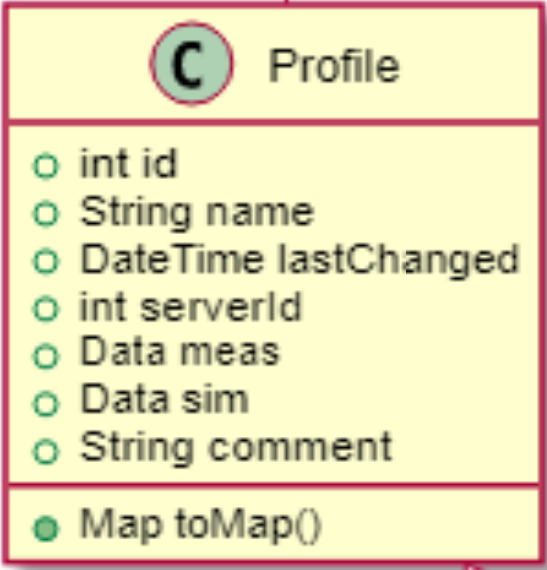
\includegraphics[width=0.5\textwidth]{../include/images/techdoc/profileClass}
		\label{img:commentTextfield}
		\caption{Aufbau der Profilklasse (\textit{profile.dart})}
	\end{figure}

	\begin{figure}[H]
		\centering
		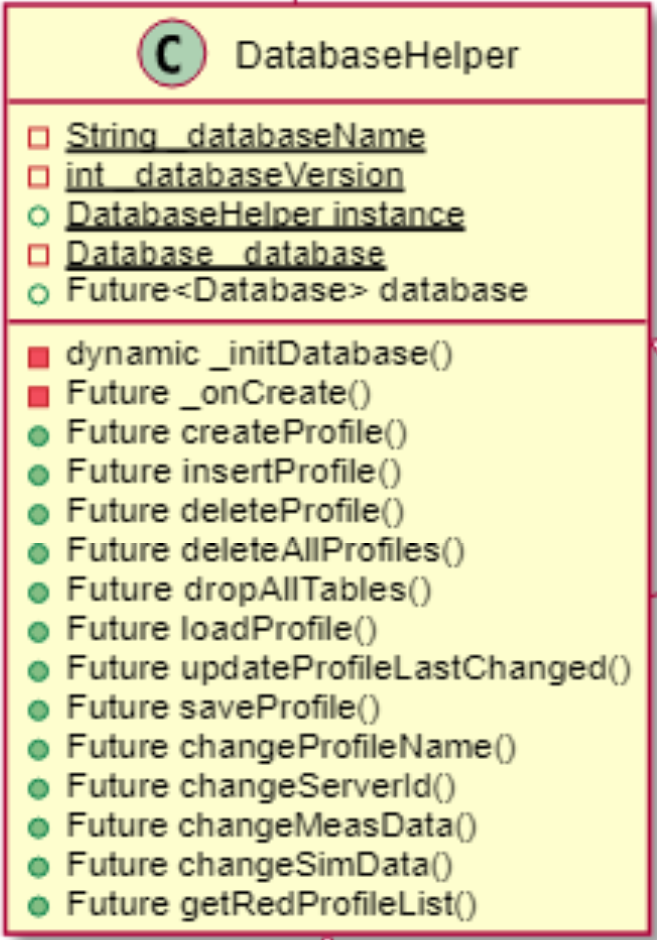
\includegraphics[width=0.5\textwidth]{../include/images/techdoc/dbHelperClass}
		\label{img:commentTextfield}
		\caption{Aufbau der Hilfsklasse (\textit{database\_helpers.dart})}
	\end{figure}

	
	\section{Speicherung der Einstellungen}
	\label{sec:speicherungEinstellungen}
	
	Die Daten zur Einstellung der App bestehen aus Präferenzen zur Sprache und zur Eingabemethode. Diese werden mithilfe des \textit{Shared preferences} Plugins (\hyperlink{https://pub.dev/packages/sqflite}{https://pub.dev/packages/sqflite}) persistent gespeichert. Da diese Daten nur sehr wenig Speicherplatz benötigen und eine Speicherung mithilfe von Shared preferences sehr einfach ist, wurde hierfür diese Technik gewählt.
	                                                                                                                                                              \hyperlink{https://pub.dev/packages/sqflite}{https://pub.dev/packages/sqflite}
	\section{Verwaltung des App-States}
	\label{sec:verwaltungAppState}
	
	- ScopedModel
	
	\section{Daten hinzufügen}
	\label{}
	
	- QR: Library
	- Vom Server: HTTP-Request (Domain, an die der Request geht)
	- 
	
	
	\section{Diagramme}
	\label{}
	
	- Library
	- KPS: Erklären, was da wichtig ist
	
	\section{}
	\label{}
	
	\section{}
	\label{}
	
	\section{}
	\label{}
	
	\section{}
	\label{}
	
	\section{}
	\label{}